\documentclass[border=14pt]{standalone}
\usepackage{tikz}
\usetikzlibrary{arrows.meta, positioning, shapes.geometric, calc}

\begin{document}
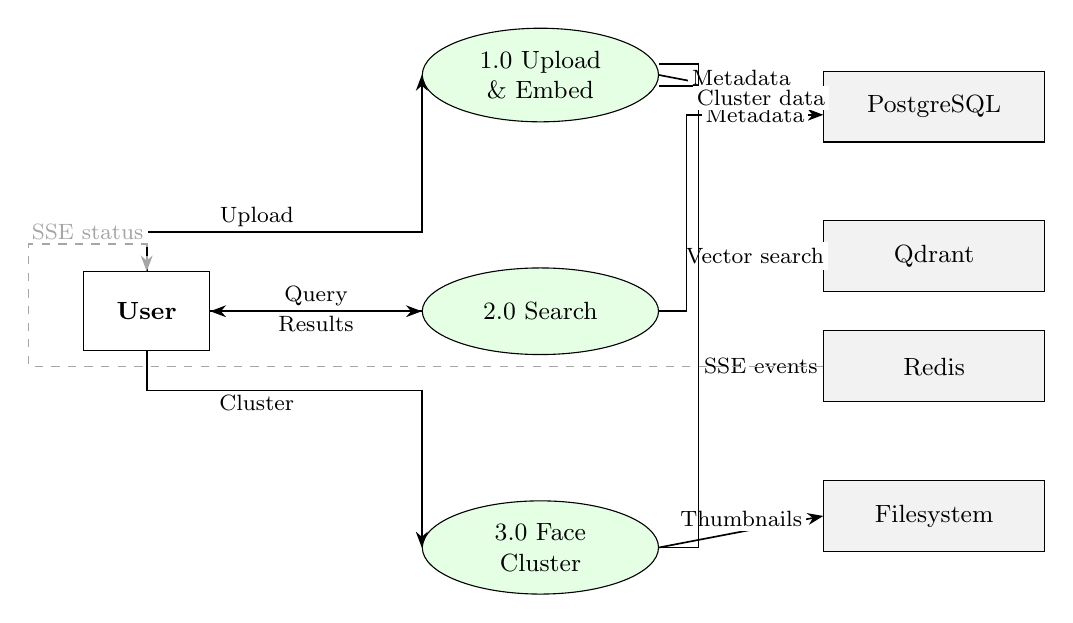
\begin{tikzpicture}[
  user/.style ={draw, rectangle, minimum width=1.6cm, minimum height=1.0cm,
                align=center, font=\small\bfseries},
  proc/.style ={draw, ellipse,  minimum width=3.0cm,  minimum height=1.1cm,
                align=center, font=\small, fill=green!10},
  store/.style={draw, rectangle,minimum width=2.8cm,  minimum height=0.9cm,
                align=center, font=\small, fill=gray!10},
  arr/.style  ={->, >=Stealth, semithick},
  sse/.style  ={->, >=Stealth, semithick, dashed, color=gray!70},
  lbl/.style  ={font=\footnotesize, fill=white, inner sep=1.5pt},
]

%% ---- Nodes ----
\node[user]  (U)  at ( 0,   0)   {User};
\node[proc]  (P1) at ( 5,   3)   {1.0 Upload\\\& Embed};
\node[proc]  (P2) at ( 5,   0)   {2.0 Search};
\node[proc]  (P3) at ( 5,  -3)   {3.0 Face\\Cluster};
\node[store] (PG) at (10,  2.6)  {PostgreSQL};
\node[store] (QD) at (10,  0.7)  {Qdrant};
\node[store] (RD) at (10, -0.7)  {Redis};
\node[store] (FS) at (10, -2.6)  {Filesystem};

%% ---- User -> Processes ----
\draw[arr] (U.north) -- ++(0,0.5) -| node[lbl,pos=0.2,above]{Upload}   (P1.west);
\draw[arr] (U.east)              -- node[lbl,above]{Query}               (P2.west);
\draw[arr] (P2.west)             -- node[lbl,below]{Results}             (U.east);
\draw[arr] (U.south) -- ++(0,-0.5) -| node[lbl,pos=0.2,below]{Cluster} (P3.west);

%% ---- P1 -> Stores (separate entry points into PG to avoid label clash) ----
\draw[arr] (P1.east) -- node[lbl,above]{Metadata}    (PG.west);
\draw[arr] ([yshift= 4pt]P1.east) -- ++(0.5,0) |- node[lbl,near end]{Embeddings} (QD.west);
\draw[arr] ([yshift=-4pt]P1.east) -- ++(0.5,0) |- node[lbl,near end]{SSE events} (RD.west);

%% ---- P2 -> Stores ----
\draw[arr] (P2.east) -- ++(0.35,0) |- node[lbl,near end]{Vector search} (QD.west);
\draw[arr] (P2.east) -- ++(0.35,0) |- node[lbl,near end]{Metadata}      ([yshift=-3pt]PG.west);

%% ---- P3 -> Stores ----
\draw[arr] (P3.east) -- node[lbl,above]{Thumbnails}  (FS.west);
\draw[arr] (P3.east) -- ++(0.5,0) |- node[lbl,near end]{Cluster data}  ([yshift=3pt]PG.west);

%% ---- SSE status: Redis.west -> left spine (x=-1.5) -> User.north ----
\draw[sse]
  (RD.west)
  -- (-1.5,-0.7)
  -- (-1.5, 0.85)
  -- node[lbl,above, pos=0.5]{SSE status}
  (U.north |- {(0, 0.85)})
  -- (U.north);

\end{tikzpicture}
\end{document}
